% Created by tikzDevice version 0.10.1 on 2016-07-30 21:03:42
% !TEX encoding = UTF-8 Unicode
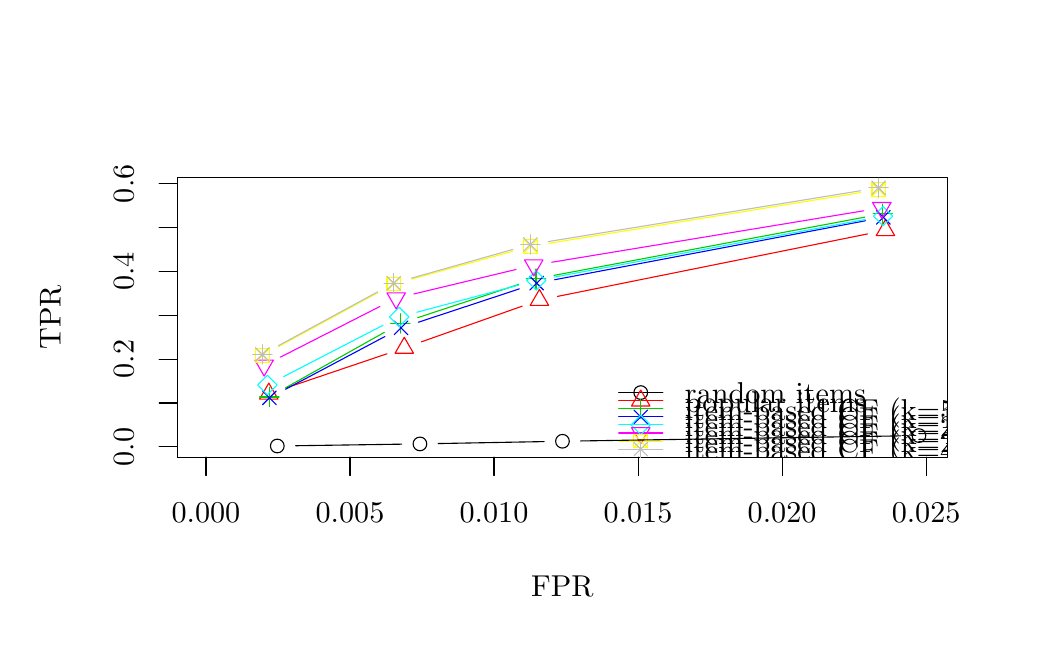
\begin{tikzpicture}[x=1pt,y=1pt]
\definecolor{fillColor}{RGB}{255,255,255}
\path[use as bounding box,fill=fillColor,fill opacity=0.00] (0,0) rectangle (360.07,222.54);
\begin{scope}
\path[clip] (  0.00,  0.00) rectangle (360.07,222.54);
\definecolor{drawColor}{RGB}{0,0,0}

\path[draw=drawColor,line width= 0.4pt,line join=round,line cap=round] ( 64.42, 67.32) -- (324.65, 67.32);

\path[draw=drawColor,line width= 0.4pt,line join=round,line cap=round] ( 64.42, 67.32) -- ( 64.42, 60.72);

\path[draw=drawColor,line width= 0.4pt,line join=round,line cap=round] (116.47, 67.32) -- (116.47, 60.72);

\path[draw=drawColor,line width= 0.4pt,line join=round,line cap=round] (168.51, 67.32) -- (168.51, 60.72);

\path[draw=drawColor,line width= 0.4pt,line join=round,line cap=round] (220.56, 67.32) -- (220.56, 60.72);

\path[draw=drawColor,line width= 0.4pt,line join=round,line cap=round] (272.60, 67.32) -- (272.60, 60.72);

\path[draw=drawColor,line width= 0.4pt,line join=round,line cap=round] (324.65, 67.32) -- (324.65, 60.72);

\node[text=drawColor,anchor=base,inner sep=0pt, outer sep=0pt, scale=  1.09] at ( 64.42, 43.56) {0.000};

\node[text=drawColor,anchor=base,inner sep=0pt, outer sep=0pt, scale=  1.09] at (116.47, 43.56) {0.005};

\node[text=drawColor,anchor=base,inner sep=0pt, outer sep=0pt, scale=  1.09] at (168.51, 43.56) {0.010};

\node[text=drawColor,anchor=base,inner sep=0pt, outer sep=0pt, scale=  1.09] at (220.56, 43.56) {0.015};

\node[text=drawColor,anchor=base,inner sep=0pt, outer sep=0pt, scale=  1.09] at (272.60, 43.56) {0.020};

\node[text=drawColor,anchor=base,inner sep=0pt, outer sep=0pt, scale=  1.09] at (324.65, 43.56) {0.025};

\path[draw=drawColor,line width= 0.4pt,line join=round,line cap=round] ( 54.12, 71.06) -- ( 54.12,166.15);

\path[draw=drawColor,line width= 0.4pt,line join=round,line cap=round] ( 54.12, 71.06) -- ( 47.52, 71.06);

\path[draw=drawColor,line width= 0.4pt,line join=round,line cap=round] ( 54.12, 86.91) -- ( 47.52, 86.91);

\path[draw=drawColor,line width= 0.4pt,line join=round,line cap=round] ( 54.12,102.76) -- ( 47.52,102.76);

\path[draw=drawColor,line width= 0.4pt,line join=round,line cap=round] ( 54.12,118.61) -- ( 47.52,118.61);

\path[draw=drawColor,line width= 0.4pt,line join=round,line cap=round] ( 54.12,134.46) -- ( 47.52,134.46);

\path[draw=drawColor,line width= 0.4pt,line join=round,line cap=round] ( 54.12,150.31) -- ( 47.52,150.31);

\path[draw=drawColor,line width= 0.4pt,line join=round,line cap=round] ( 54.12,166.15) -- ( 47.52,166.15);

\node[text=drawColor,rotate= 90.00,anchor=base,inner sep=0pt, outer sep=0pt, scale=  1.09] at ( 38.28, 71.06) {0.0};

\node[text=drawColor,rotate= 90.00,anchor=base,inner sep=0pt, outer sep=0pt, scale=  1.09] at ( 38.28,102.76) {0.2};

\node[text=drawColor,rotate= 90.00,anchor=base,inner sep=0pt, outer sep=0pt, scale=  1.09] at ( 38.28,134.46) {0.4};

\node[text=drawColor,rotate= 90.00,anchor=base,inner sep=0pt, outer sep=0pt, scale=  1.09] at ( 38.28,166.15) {0.6};

\path[draw=drawColor,line width= 0.4pt,line join=round,line cap=round] ( 54.12, 67.32) --
	(332.35, 67.32) --
	(332.35,168.42) --
	( 54.12,168.42) --
	( 54.12, 67.32);
\end{scope}
\begin{scope}
\path[clip] (  0.00,  0.00) rectangle (360.07,222.54);
\definecolor{drawColor}{RGB}{0,0,0}

\node[text=drawColor,anchor=base,inner sep=0pt, outer sep=0pt, scale=  1.09] at (193.24, 17.16) {FPR};

\node[text=drawColor,rotate= 90.00,anchor=base,inner sep=0pt, outer sep=0pt, scale=  1.09] at ( 11.88,117.87) {TPR};
\end{scope}
\begin{scope}
\path[clip] ( 54.12, 67.32) rectangle (332.35,168.42);
\definecolor{drawColor}{RGB}{0,0,0}

\path[draw=drawColor,line width= 0.4pt,line join=round,line cap=round] (213.56, 90.68) -- (229.51, 90.68);
\definecolor{drawColor}{RGB}{255,0,0}

\path[draw=drawColor,line width= 0.4pt,line join=round,line cap=round] (213.56, 87.76) -- (229.51, 87.76);
\definecolor{drawColor}{RGB}{0,205,0}

\path[draw=drawColor,line width= 0.4pt,line join=round,line cap=round] (213.56, 84.84) -- (229.51, 84.84);
\definecolor{drawColor}{RGB}{0,0,255}

\path[draw=drawColor,line width= 0.4pt,line join=round,line cap=round] (213.56, 81.92) -- (229.51, 81.92);
\definecolor{drawColor}{RGB}{0,255,255}

\path[draw=drawColor,line width= 0.4pt,line join=round,line cap=round] (213.56, 79.00) -- (229.51, 79.00);
\definecolor{drawColor}{RGB}{255,0,255}

\path[draw=drawColor,line width= 0.4pt,line join=round,line cap=round] (213.56, 76.08) -- (229.51, 76.08);
\definecolor{drawColor}{RGB}{255,255,0}

\path[draw=drawColor,line width= 0.4pt,line join=round,line cap=round] (213.56, 73.16) -- (229.51, 73.16);
\definecolor{drawColor}{RGB}{190,190,190}

\path[draw=drawColor,line width= 0.4pt,line join=round,line cap=round] (213.56, 70.24) -- (229.51, 70.24);
\definecolor{drawColor}{RGB}{0,0,0}

\path[draw=drawColor,line width= 0.4pt,line join=round,line cap=round] (221.53, 90.68) circle (  2.47);
\definecolor{drawColor}{RGB}{255,0,0}

\path[draw=drawColor,line width= 0.4pt,line join=round,line cap=round] (221.53, 91.61) --
	(224.87, 85.84) --
	(218.20, 85.84) --
	(221.53, 91.61);
\definecolor{drawColor}{RGB}{0,205,0}

\path[draw=drawColor,line width= 0.4pt,line join=round,line cap=round] (218.03, 84.84) -- (225.03, 84.84);

\path[draw=drawColor,line width= 0.4pt,line join=round,line cap=round] (221.53, 81.34) -- (221.53, 88.34);
\definecolor{drawColor}{RGB}{0,0,255}

\path[draw=drawColor,line width= 0.4pt,line join=round,line cap=round] (219.06, 79.45) -- (224.01, 84.40);

\path[draw=drawColor,line width= 0.4pt,line join=round,line cap=round] (219.06, 84.40) -- (224.01, 79.45);
\definecolor{drawColor}{RGB}{0,255,255}

\path[draw=drawColor,line width= 0.4pt,line join=round,line cap=round] (218.03, 79.00) --
	(221.53, 82.50) --
	(225.03, 79.00) --
	(221.53, 75.50) --
	(218.03, 79.00);
\definecolor{drawColor}{RGB}{255,0,255}

\path[draw=drawColor,line width= 0.4pt,line join=round,line cap=round] (221.53, 72.23) --
	(224.87, 78.01) --
	(218.20, 78.01) --
	(221.53, 72.23);
\definecolor{drawColor}{RGB}{255,255,0}

\path[draw=drawColor,line width= 0.4pt,line join=round,line cap=round] (219.06, 70.69) rectangle (224.01, 75.64);

\path[draw=drawColor,line width= 0.4pt,line join=round,line cap=round] (219.06, 70.69) -- (224.01, 75.64);

\path[draw=drawColor,line width= 0.4pt,line join=round,line cap=round] (219.06, 75.64) -- (224.01, 70.69);
\definecolor{drawColor}{RGB}{190,190,190}

\path[draw=drawColor,line width= 0.4pt,line join=round,line cap=round] (219.06, 67.77) -- (224.01, 72.72);

\path[draw=drawColor,line width= 0.4pt,line join=round,line cap=round] (219.06, 72.72) -- (224.01, 67.77);

\path[draw=drawColor,line width= 0.4pt,line join=round,line cap=round] (218.03, 70.24) -- (225.03, 70.24);

\path[draw=drawColor,line width= 0.4pt,line join=round,line cap=round] (221.53, 66.74) -- (221.53, 73.74);
\definecolor{drawColor}{RGB}{0,0,0}

\node[text=drawColor,anchor=base west,inner sep=0pt, outer sep=0pt, scale=  1.09] at (237.48, 86.57) {random items};

\node[text=drawColor,anchor=base west,inner sep=0pt, outer sep=0pt, scale=  1.09] at (237.48, 83.65) {popular items};

\node[text=drawColor,anchor=base west,inner sep=0pt, outer sep=0pt, scale=  1.09] at (237.48, 80.73) {item-based CF (k=5)};

\node[text=drawColor,anchor=base west,inner sep=0pt, outer sep=0pt, scale=  1.09] at (237.48, 77.81) {item-based CF (k=10)};

\node[text=drawColor,anchor=base west,inner sep=0pt, outer sep=0pt, scale=  1.09] at (237.48, 74.89) {item-based CF (k=20)};

\node[text=drawColor,anchor=base west,inner sep=0pt, outer sep=0pt, scale=  1.09] at (237.48, 71.97) {item-based CF (k=40)};

\node[text=drawColor,anchor=base west,inner sep=0pt, outer sep=0pt, scale=  1.09] at (237.48, 69.05) {item-based CF (k=200)};

\node[text=drawColor,anchor=base west,inner sep=0pt, outer sep=0pt, scale=  1.09] at (237.48, 66.13) {item-based CF (k=402)};

\path[draw=drawColor,line width= 0.4pt,line join=round,line cap=round] ( 96.80, 71.47) -- (135.14, 72.04);

\path[draw=drawColor,line width= 0.4pt,line join=round,line cap=round] (148.34, 72.26) -- (186.64, 72.97);

\path[draw=drawColor,line width= 0.4pt,line join=round,line cap=round] (199.84, 73.20) -- (315.45, 75.03);

\path[draw=drawColor,line width= 0.4pt,line join=round,line cap=round] ( 90.20, 71.38) circle (  2.47);

\path[draw=drawColor,line width= 0.4pt,line join=round,line cap=round] (141.74, 72.13) circle (  2.47);

\path[draw=drawColor,line width= 0.4pt,line join=round,line cap=round] (193.24, 73.09) circle (  2.47);

\path[draw=drawColor,line width= 0.4pt,line join=round,line cap=round] (322.05, 75.14) circle (  2.47);
\definecolor{drawColor}{RGB}{255,0,0}

\path[draw=drawColor,line width= 0.4pt,line join=round,line cap=round] ( 93.38, 92.37) -- (129.83,104.70);

\path[draw=drawColor,line width= 0.4pt,line join=round,line cap=round] (142.30,109.02) -- (178.70,121.91);

\path[draw=drawColor,line width= 0.4pt,line join=round,line cap=round] (191.39,125.42) -- (303.49,148.01);

\path[draw=drawColor,line width= 0.4pt,line join=round,line cap=round] ( 87.13, 94.10) --
	( 90.46, 88.33) --
	( 83.79, 88.33) --
	( 87.13, 94.10);

\path[draw=drawColor,line width= 0.4pt,line join=round,line cap=round] (136.08,110.67) --
	(139.42,104.89) --
	(132.75,104.89) --
	(136.08,110.67);

\path[draw=drawColor,line width= 0.4pt,line join=round,line cap=round] (184.92,127.96) --
	(188.25,122.19) --
	(181.59,122.19) --
	(184.92,127.96);

\path[draw=drawColor,line width= 0.4pt,line join=round,line cap=round] (309.96,153.16) --
	(313.29,147.39) --
	(306.62,147.39) --
	(309.96,153.16);
\definecolor{drawColor}{RGB}{0,205,0}

\path[draw=drawColor,line width= 0.4pt,line join=round,line cap=round] ( 93.07, 92.33) -- (128.89,112.45);

\path[draw=drawColor,line width= 0.4pt,line join=round,line cap=round] (140.91,117.74) -- (177.40,129.75);

\path[draw=drawColor,line width= 0.4pt,line join=round,line cap=round] (190.15,133.03) -- (302.50,154.07);

\path[draw=drawColor,line width= 0.4pt,line join=round,line cap=round] ( 83.81, 89.10) -- ( 90.81, 89.10);

\path[draw=drawColor,line width= 0.4pt,line join=round,line cap=round] ( 87.31, 85.60) -- ( 87.31, 92.60);

\path[draw=drawColor,line width= 0.4pt,line join=round,line cap=round] (131.14,115.68) -- (138.14,115.68);

\path[draw=drawColor,line width= 0.4pt,line join=round,line cap=round] (134.64,112.18) -- (134.64,119.18);

\path[draw=drawColor,line width= 0.4pt,line join=round,line cap=round] (180.17,131.82) -- (187.17,131.82);

\path[draw=drawColor,line width= 0.4pt,line join=round,line cap=round] (183.67,128.32) -- (183.67,135.32);

\path[draw=drawColor,line width= 0.4pt,line join=round,line cap=round] (305.48,155.28) -- (312.48,155.28);

\path[draw=drawColor,line width= 0.4pt,line join=round,line cap=round] (308.98,151.78) -- (308.98,158.78);
\definecolor{drawColor}{RGB}{0,0,255}

\path[draw=drawColor,line width= 0.4pt,line join=round,line cap=round] ( 93.19, 91.88) -- (129.08,110.93);

\path[draw=drawColor,line width= 0.4pt,line join=round,line cap=round] (141.18,116.10) -- (177.66,128.15);

\path[draw=drawColor,line width= 0.4pt,line join=round,line cap=round] (190.41,131.45) -- (302.71,152.76);

\path[draw=drawColor,line width= 0.4pt,line join=round,line cap=round] ( 84.89, 86.31) -- ( 89.84, 91.26);

\path[draw=drawColor,line width= 0.4pt,line join=round,line cap=round] ( 84.89, 91.26) -- ( 89.84, 86.31);

\path[draw=drawColor,line width= 0.4pt,line join=round,line cap=round] (132.43,111.56) -- (137.38,116.51);

\path[draw=drawColor,line width= 0.4pt,line join=round,line cap=round] (132.43,116.51) -- (137.38,111.56);

\path[draw=drawColor,line width= 0.4pt,line join=round,line cap=round] (181.45,127.74) -- (186.40,132.69);

\path[draw=drawColor,line width= 0.4pt,line join=round,line cap=round] (181.45,132.69) -- (186.40,127.74);

\path[draw=drawColor,line width= 0.4pt,line join=round,line cap=round] (306.72,151.52) -- (311.67,156.47);

\path[draw=drawColor,line width= 0.4pt,line join=round,line cap=round] (306.72,156.47) -- (311.67,151.52);
\definecolor{drawColor}{RGB}{0,255,255}

\path[draw=drawColor,line width= 0.4pt,line join=round,line cap=round] ( 92.48, 96.44) -- (128.39,114.99);

\path[draw=drawColor,line width= 0.4pt,line join=round,line cap=round] (140.64,119.71) -- (177.39,129.50);

\path[draw=drawColor,line width= 0.4pt,line join=round,line cap=round] (190.26,132.40) -- (302.63,153.23);

\path[draw=drawColor,line width= 0.4pt,line join=round,line cap=round] ( 83.11, 93.42) --
	( 86.61, 96.92) --
	( 90.11, 93.42) --
	( 86.61, 89.92) --
	( 83.11, 93.42);

\path[draw=drawColor,line width= 0.4pt,line join=round,line cap=round] (130.76,118.02) --
	(134.26,121.52) --
	(137.76,118.02) --
	(134.26,114.51) --
	(130.76,118.02);

\path[draw=drawColor,line width= 0.4pt,line join=round,line cap=round] (180.27,131.19) --
	(183.77,134.69) --
	(187.27,131.19) --
	(183.77,127.69) --
	(180.27,131.19);

\path[draw=drawColor,line width= 0.4pt,line join=round,line cap=round] (305.62,154.44) --
	(309.12,157.94) --
	(312.62,154.44) --
	(309.12,150.94) --
	(305.62,154.44);
\definecolor{drawColor}{RGB}{255,0,255}

\path[draw=drawColor,line width= 0.4pt,line join=round,line cap=round] ( 91.34,103.49) -- (127.27,121.79);

\path[draw=drawColor,line width= 0.4pt,line join=round,line cap=round] (139.57,126.32) -- (176.45,135.16);

\path[draw=drawColor,line width= 0.4pt,line join=round,line cap=round] (189.38,137.77) -- (302.12,156.37);

\path[draw=drawColor,line width= 0.4pt,line join=round,line cap=round] ( 85.46, 96.65) --
	( 88.79,102.42) --
	( 82.12,102.42) --
	( 85.46, 96.65);

\path[draw=drawColor,line width= 0.4pt,line join=round,line cap=round] (133.16,120.93) --
	(136.49,126.71) --
	(129.82,126.71) --
	(133.16,120.93);

\path[draw=drawColor,line width= 0.4pt,line join=round,line cap=round] (182.87,132.84) --
	(186.20,138.62) --
	(179.54,138.62) --
	(182.87,132.84);

\path[draw=drawColor,line width= 0.4pt,line join=round,line cap=round] (308.63,153.59) --
	(311.97,159.37) --
	(305.30,159.37) --
	(308.63,153.59);
\definecolor{drawColor}{RGB}{255,255,0}

\path[draw=drawColor,line width= 0.4pt,line join=round,line cap=round] ( 90.66,107.29) -- (126.52,126.75);

\path[draw=drawColor,line width= 0.4pt,line join=round,line cap=round] (138.68,131.66) -- (175.39,141.79);

\path[draw=drawColor,line width= 0.4pt,line join=round,line cap=round] (188.27,144.61) -- (301.04,162.97);

\path[draw=drawColor,line width= 0.4pt,line join=round,line cap=round] ( 82.39,101.67) rectangle ( 87.34,106.62);

\path[draw=drawColor,line width= 0.4pt,line join=round,line cap=round] ( 82.39,101.67) -- ( 87.34,106.62);

\path[draw=drawColor,line width= 0.4pt,line join=round,line cap=round] ( 82.39,106.62) -- ( 87.34,101.67);

\path[draw=drawColor,line width= 0.4pt,line join=round,line cap=round] (129.85,127.43) rectangle (134.80,132.38);

\path[draw=drawColor,line width= 0.4pt,line join=round,line cap=round] (129.85,127.43) -- (134.80,132.38);

\path[draw=drawColor,line width= 0.4pt,line join=round,line cap=round] (129.85,132.38) -- (134.80,127.43);

\path[draw=drawColor,line width= 0.4pt,line join=round,line cap=round] (179.28,141.07) rectangle (184.23,146.02);

\path[draw=drawColor,line width= 0.4pt,line join=round,line cap=round] (179.28,141.07) -- (184.23,146.02);

\path[draw=drawColor,line width= 0.4pt,line join=round,line cap=round] (179.28,146.02) -- (184.23,141.07);

\path[draw=drawColor,line width= 0.4pt,line join=round,line cap=round] (305.08,161.56) rectangle (310.03,166.51);

\path[draw=drawColor,line width= 0.4pt,line join=round,line cap=round] (305.08,161.56) -- (310.03,166.51);

\path[draw=drawColor,line width= 0.4pt,line join=round,line cap=round] (305.08,166.51) -- (310.03,161.56);
\definecolor{drawColor}{RGB}{190,190,190}

\path[draw=drawColor,line width= 0.4pt,line join=round,line cap=round] ( 90.61,107.63) -- (126.47,127.07);

\path[draw=drawColor,line width= 0.4pt,line join=round,line cap=round] (138.62,132.01) -- (175.30,142.40);

\path[draw=drawColor,line width= 0.4pt,line join=round,line cap=round] (188.16,145.26) -- (300.94,163.62);

\path[draw=drawColor,line width= 0.4pt,line join=round,line cap=round] ( 82.33,102.00) -- ( 87.28,106.95);

\path[draw=drawColor,line width= 0.4pt,line join=round,line cap=round] ( 82.33,106.95) -- ( 87.28,102.00);

\path[draw=drawColor,line width= 0.4pt,line join=round,line cap=round] ( 81.31,104.48) -- ( 88.31,104.48);

\path[draw=drawColor,line width= 0.4pt,line join=round,line cap=round] ( 84.81,100.98) -- ( 84.81,107.98);

\path[draw=drawColor,line width= 0.4pt,line join=round,line cap=round] (129.80,127.74) -- (134.75,132.69);

\path[draw=drawColor,line width= 0.4pt,line join=round,line cap=round] (129.80,132.69) -- (134.75,127.74);

\path[draw=drawColor,line width= 0.4pt,line join=round,line cap=round] (128.77,130.21) -- (135.77,130.21);

\path[draw=drawColor,line width= 0.4pt,line join=round,line cap=round] (132.27,126.71) -- (132.27,133.71);

\path[draw=drawColor,line width= 0.4pt,line join=round,line cap=round] (179.17,141.72) -- (184.12,146.67);

\path[draw=drawColor,line width= 0.4pt,line join=round,line cap=round] (179.17,146.67) -- (184.12,141.72);

\path[draw=drawColor,line width= 0.4pt,line join=round,line cap=round] (178.15,144.20) -- (185.15,144.20);

\path[draw=drawColor,line width= 0.4pt,line join=round,line cap=round] (181.65,140.69) -- (181.65,147.70);

\path[draw=drawColor,line width= 0.4pt,line join=round,line cap=round] (304.98,162.20) -- (309.93,167.15);

\path[draw=drawColor,line width= 0.4pt,line join=round,line cap=round] (304.98,167.15) -- (309.93,162.20);

\path[draw=drawColor,line width= 0.4pt,line join=round,line cap=round] (303.95,164.68) -- (310.95,164.68);

\path[draw=drawColor,line width= 0.4pt,line join=round,line cap=round] (307.45,161.18) -- (307.45,168.18);
\end{scope}
\end{tikzpicture}
